\documentclass[11pt,a4paper]{article}
\usepackage[T1]{fontenc}
\usepackage[utf8]{inputenc}
\usepackage{lmodern}
\usepackage[a4paper,margin=2.2cm]{geometry}
\usepackage{microtype}
\usepackage{amsmath}
\usepackage{graphicx}
\usepackage{booktabs}
\usepackage{tabularx}
\usepackage{array}
\usepackage{siunitx}
\usepackage[font=small,labelfont=bf]{caption}
\usepackage{xcolor}
\usepackage{xurl}
\usepackage[section]{placeins}
\usepackage{float}
\usepackage[colorlinks=true,linkcolor=blue!50!black,citecolor=blue!50!black,urlcolor=blue!50!black]{hyperref}

\sisetup{range-phrase={\text{ to }},range-units=single,per-mode=symbol}
\newcolumntype{L}{>{\raggedright\arraybackslash}X}
\newcommand{\eps}{\varepsilon}
\newcommand{\file}[1]{\nolinkurl{#1}}
\newcommand{\elec}{e$^-$}

\title{Single-atom detection versus camera parameters at 852\,nm\\[4pt]
\large P1 interim technical report: validation, camera presets, sensitivity and Sobol analyses}
\author{CAQSAT lab, Department of Physics, IIT Madras}
\date{16 October 2026 \quad (status: interim)}

\begin{document}
\maketitle

\noindent This report covers the shared package \file{camsim_common} and project P1 through the
validation stage, the camera presets and sensitivity study with the measured V1 point-spread function
(PSF), and two interim Sobol analyses. It supersedes the summary sections of
\file{reports/p1_production_note.md}, which uses a diffraction-limited PSF. Detailed results are in
\file{reports/p1_validation.md}, \file{reports/p1_sobol_interim_n256.md} and
\file{reports/p1_sobol_camera_n256.md}. All results are simulations (SIM) unless marked otherwise, and
every SIM value should be reviewed before submission.

\section*{Summary}

We built a semi-analytic model that maps a camera description (\file{SensorModel}) and the photon
budget and loss of a trapped Cs atom to the false-positive (FP) and false-negative (FN) rates of
single-site occupancy detection, and from them to the imaging time needed for a target infidelity
$\eps$. The model reproduces the FN rate of Manetsch \textit{et al.}~\cite{manetsch} to within 11\% and
the readout statistics of Picken \textit{et al.}~\cite{picken}, but under-predicts the FP rate of
Manetsch \textit{et al.} by a factor of 14, which we attribute to events outside a camera model.

In a reference scenario anchored on Manetsch \textit{et al.} (NA 0.55, measured PSF of FWHM
\SI{1.70}{\micro\metre}, 2.7\% of scattered photons reaching the camera), five low-noise CMOS
configurations reach $\eps = 10^{-4}$ in \SIrange{40}{44}{\milli\second} with a matched-filter
classifier, and an EMCCD in multi-frame photon counting in \SI{34}{\milli\second}. The Prime BSI Express
in CMS mode needs \SI{28.4}{\milli\second} for $10^{-3}$ and \SI{41.3}{\milli\second} for $10^{-4}$,
within 20\% of the best camera in the set. Cameras with a quantum efficiency (QE) at 852\,nm below 0.25
need 2.5 to 4 times longer than the CMOS group or do not reach $10^{-4}$.

Over the camera-side parameter space, the imaging time is set by QE and read noise, which act
separably: at the reference background and 1 pixel per PSF FWHM, $t$ is proportional to $1/\mathrm{QE}$
times a read-noise factor that is 0.77 at 0.1\,\elec, 0.84 at 0.5\,\elec, 1 at 1.0\,\elec{} and 1.42 at
2.0\,\elec{} (for $10^{-4}$). Hence QE is the main lever for a Stage~1 sensor, and a read-noise median
below 0.5\,\elec{} gains less than 10\%. Two inputs that carry little variance globally matter at the
operating point: a 2\% fraction of pixels at five times the median read noise slows a 1\,\elec{} camera
by 42\%, and the loss per scattered photon decides whether $10^{-4}$ is reachable at all. NA and atom
loss, which are properties of the experiment, outweigh every camera parameter.

The main limitations are (i)~the unexplained FP floor of the V1 experiment, (ii)~an assumed two-class
read-noise tail in place of a measured distribution, and (iii)~a single reference scenario at 852\,nm;
Rb at 780\,nm and array crosstalk are not yet treated.

\section{Scope and what was run}

The P1 brief asks three questions: (i)~which sensor parameters set the infidelity and imaging time,
and with what sensitivity; (ii)~what minimum specification reaches $10^{-3}$ and $10^{-4}$ within a
given imaging time and loss budget (the Stage~1 camera specification); and (iii)~how the lab should
operate the Prime BSI Express. This report gives interim answers to (i) and (iii) and the elements
of (ii).

We ran (a)~validation stages V1 to V3 with a convergence study; (b)~eleven camera presets at seven
pixel samplings, with the diffraction-limited and with the measured PSF; (c)~a sensitivity study of
the preset results to their uncertain inputs; (d)~a reduced generic CMOS-class sweep of 750 points
with the diffraction-limited PSF; (e)~Sobol analyses at $N = 256$ of an 8-parameter design (camera
parameters, NA and loss) and of a 6-parameter camera-only design (NA and loss fixed).
Table~\ref{tab:cost} lists the cost of each.

\section{Model and validation}

Here, an atom present for the full exposure $t$ yields
\begin{equation}
  \mu = R\, t\, \eta_\mathrm{cam}\, \mathrm{QE}
\end{equation}
detected photoelectrons, with $R$ the scattering rate,
$\eta_\mathrm{cam} = \eta_\mathrm{coll}(\mathrm{NA})\,\eta_\mathrm{opt}$ the fraction of scattered
photons reaching the sensor and QE the quantum efficiency at 852\,nm. Loss during imaging truncates
the exposure; model~A uses a constant loss probability per scattered photon, model~B a 3D Langevin
walk in the trap. Per-pixel counts are Poisson in signal plus background, convolved with a
Gaussian-mixture read-noise model (core plus tail pixels) or, for an EMCCD, a gamma-distributed
multiplication register with clock-induced charge (CIC)~\cite{basden}. Site classification uses a box
sum, a matched filter with Fisher-optimal pixel weights, or a per-pixel Bayesian likelihood ratio.
Count distributions are computed exactly on a lattice or, for linear statistics, from characteristic
functions (within 2\% of the lattice result in optimal infidelity, about $10^3$ times faster), and
cross-checked against brute-force and importance-sampled Monte Carlo at $10^{-3}$. Thresholds are
optimised per site and averaged over $3\times3$ sub-pixel site positions (within 1.1\% of a $9\times9$
average).

\begin{table}[htbp]
\centering
\caption{Validation results. Details and residuals in \file{reports/p1_validation.md}.}
\label{tab:validation}
\footnotesize
\begin{tabularx}{\textwidth}{@{}l L L l@{}}
\toprule
stage & target (source) & model result & status \\
\midrule
V1 & FN $5.50\times10^{-5}$, FP $7.01\times10^{-5}$, ORCA-Quest, 80\,ms~\cite{manetsch} &
FN $4.91\times10^{-5}$ (empirical rate spread) to $5.73\times10^{-5}$ (Gaussian); FP $4.85\times10^{-6}$ &
FN reproduced; FP $14\times$ low \\
V1 & dependence on loss-time profile at fixed survival 0.999864 &
FN $-42\%$ (model~B, late losses) to $+10\%$ (model~B, early escape) relative to model~A & quantified \\
V2 & Zyla 5.5, 40\,ms, readout error $< 8\times10^{-7}$~\cite{picken} &
fitted gains 0.381 and 0.368\,\elec/ADU (agree between traps); Poisson readout error 2.9 to 4.0 times
their Gaussian estimate ($9.55\times10^{-7}$ for trap~1) & reproduced; bound marginal \\
V2 & sCMOS vs EMCCD SNR table (their Table~I) &
all cells to 0.05 except two EMCCD 852\,nm cells, consistent with QE 0.55 instead of 0.60 & reproduced \\
V3 & Poisson limit; EMCCD excess noise $F^2 \to 2$~\cite{basden} &
relative error $4.42\times10^{-14}$; $F^2 = 1.972$ at gain 1000, 512 stages & pass \\
\bottomrule
\end{tabularx}
\end{table}

The V1 FP excess is visible directly in the digitised histogram: between 32 and 42 photons the
measured background tail lies 2 to 3 times above any Poisson-plus-read-noise model consistent with the
background width. We read this as a floor set by events outside the camera, for example atoms entering
during imaging. This has a direct consequence for the present work: at the $10^{-4}$ level, a real
experiment may be limited by non-camera errors that no camera choice removes.

\section{Reference scenario}
\label{sec:scenario}

The reference scenario (\file{configs/production/reference_cs.yaml}) is derived from the V1 fit: Cs
D2 at 852\,nm~\cite{steck}; scattering rate \SI{72.3e3}{\per\second}; NA 0.55 with
$\eta_\mathrm{opt} = 0.327$ (2.7\% of scattered photons to the camera, as in V1); loss
$2.35\times10^{-8}$ per scattered photon (V1 survival, model~A); site-to-site rate spread 12.3\% rms
(V1 Ext.\ Data Fig.~4d); background 4.76\,\elec/px/s at the V1 pixel
(\SI{0.902}{\micro\metre} in the object plane, QE 0.44), scaled with pixel area and QE; filling 0.5.
The PSF is a Gaussian of $1/e^2$ radius \SI{1.44}{\micro\metre} at NA 0.55 (FWHM
\SI{1.70}{\micro\metre}), derived from the waist stated by Manetsch \textit{et al.} with the pixel
variance removed, and scaled as $1/\mathrm{NA}$ when NA is varied. Its FWHM is 2.1 times that of the
diffraction-limited vectorial PSF (\SI{0.82}{\micro\metre}). Survival is not limiting in this
scenario: the loss rate is \SI{1.7e-3}{\per\second}, so survival stays above 0.99 up to 5.9\,s
(DERIVED: $0.01005/(2.35\times10^{-8}\times\SI{72.3e3}{\per\second})$).

\section{Camera presets}

\begin{table}[htbp]
\centering
\caption{Presets at their best pixel sampling, measured PSF. Matched filter; photon counting uses an
SNR-optimal box over frames at 670\,fps (128$\times$128 crop); HCG: high conversion gain. QE at 852\,nm digitised from vendor
typical curves (DATA, about $\pm1.5$ to 2\%). Magnification for the V1 PSF (FWHM
\SI{1.70}{\micro\metre}). n/r: not reached within 300\,ms with survival $\geq 0.99$. The last column
gives $t(10^{-4})$ with the diffraction-limited vectorial PSF, each at its own best sampling.}
\label{tab:presets}
\footnotesize
\setlength{\tabcolsep}{2.8pt}
\begin{tabular}{@{}l l c c c c c c c@{}}
\toprule
camera & mode & QE & read noise & best & magni- & $t(10^{-3})$ & $t(10^{-4})$ & $t(10^{-4})$ \\
 & & 852\,nm & med./rms (\elec) & px/FWHM & fication & (ms) & (ms) & diffr.\ (ms) \\
\midrule
iXon Ultra 888 EXF & photon counting & 0.608 & EM $\times$1000 & 1.4 & 10.7 & 21.9 & 34.3 & 29.6 \\
ORCA-Fusion BT & ultra quiet & 0.464 & 0.60/0.70 & 1.0 & 3.8 & 26.7 & 39.7 & 36.9 \\
ORCA-Quest 2 & ultra quiet (PNR) & 0.384 & 0.25/0.30 & 1.4 & 3.8 & 26.4 & 40.2 & 35.7 \\
Prime BSI Express & CMS (100\,MHz) & 0.485 & 1.00/1.00 & 1.0 & 3.8 & 28.4 & 41.3 & 37.5 \\
ORCA-Quest 2 & standard & 0.384 & 0.39/0.43 & 1.0 & 2.7 & 27.9 & 42.6 & 37.9 \\
Marana 4.2B-6 & low noise 12-bit & 0.470 & 1.10/1.10 & 1.0 & 3.8 & 30.3 & 43.6 & 39.6 \\
iXon Ultra 888 EXF & analog & 0.608 & EM $\times$1000 & 3.0 & 23.0 & 30.2 & 48.1 & 42.5 \\
Prime BSI Express & Speed (200\,MHz) & 0.485 & 1.60/1.60 & 0.7 & 2.7 & 34.0 & 49.3 & 46.3 \\
QHY268M (IMX571) & HG-2CMS, g.\,100 & 0.208 & 1.19/1.19 & 0.7 & 1.6 & 68.8 & 104.2 & 94.4 \\
Zyla 5.5 & global shutter & 0.249 & 2.30/2.50 & 0.5 & 1.9 & 94.6 & 156.2 & 154.2 \\
Blackfly S (IMX425) & HCG & 0.186 & 4.69/4.69 & 0.35 & 1.9 & 179.1 & n/r & 299.6 \\
\bottomrule
\end{tabular}
\end{table}

\begin{figure}[htbp]
\centering
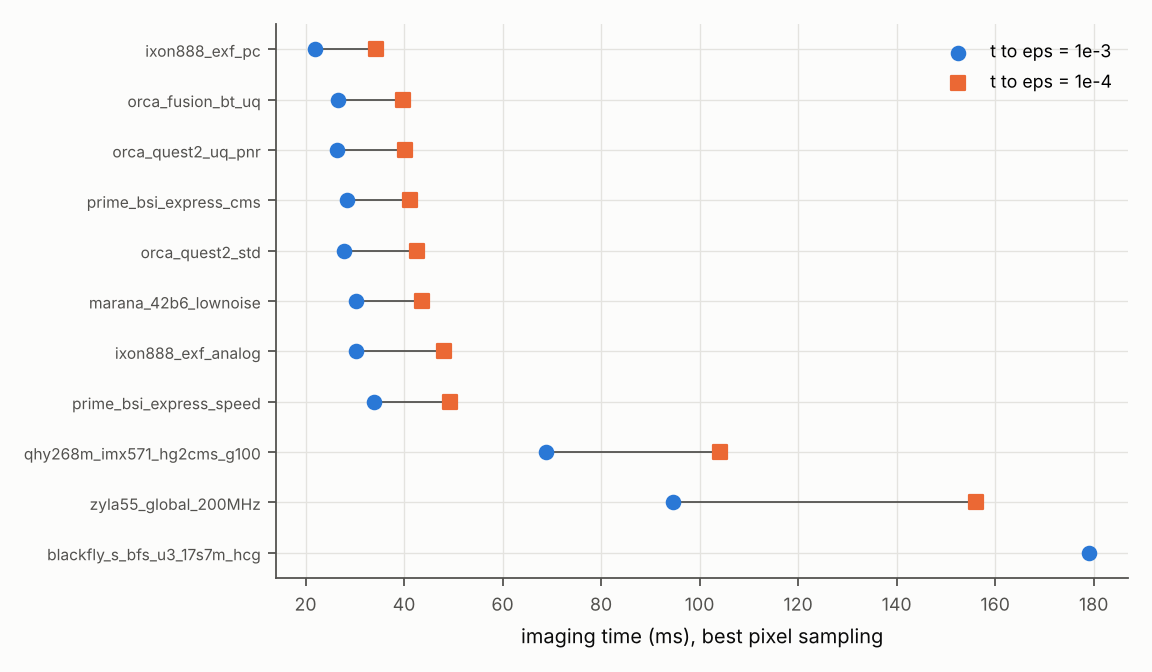
\includegraphics[width=0.82\textwidth]{../figures/prod_presets_measpsf.png}
\caption{Imaging time to $\eps = 10^{-3}$ (circles) and $10^{-4}$ (squares) for each preset at its best
pixel sampling (0.35 to 3\,px per FWHM), reference Cs scenario (Sec.~\ref{sec:scenario}) with the
measured V1 PSF. Characteristic-function engine with per-site matched filter; EMCCD photon counting
uses Poisson-binomial counts over an SNR-optimal box with frames at 670\,fps. Error rates averaged over
$3\times3$ sub-pixel site positions, threshold optimised per site, filling 0.5. The Blackfly~S does not
reach $10^{-4}$ within 300\,ms. Data: \file{runs/production/prod_presets/prod_presets.h5}.}
\label{fig:presets}
\end{figure}

As can be seen from Table~\ref{tab:presets} and Fig.~\ref{fig:presets}, the measured PSF, although
2.1 times wider than the diffraction limit, lengthens the imaging time by only 1 to 16\%. This is
because the best magnification changes little (3.8 instead of 4.0 for the Prime BSI Express): the
optimal sampling moves from about 0.5 to about 1\,px per FWHM, and the wider PSF costs only the read
noise and background of the additional pixels in the classifier window. The ranking is unchanged
except that the ORCA-Fusion BT and the ORCA-Quest~2 in PNR mode exchange places, a difference of
1.3\%. Three remarks. (i)~The iXon advantage requires photon counting over many short frames (26 frames
in 40\,ms for a $128\times128$ crop); in analog mode the excess noise factor ($F^2 = 1.97$) cancels its
QE advantage. (ii)~With the QE of 0.44 stated by Manetsch \textit{et al.} for their ORCA-Quest, instead
of 0.384 from the Quest~2 typical curve, the Quest~2 times would fall by about 13\% ($t$ roughly
proportional to $1/\mathrm{QE}$).\footnote{The vendor's typical curve for the original ORCA-Quest
(C15550-20UP) gives 0.396 at 852\,nm, so the 0.44 of Ref.~\cite{manetsch} may reflect a particular unit
or a different definition; we have not resolved this.} (iii)~Differences below about 5\% between presets
are within the QE uncertainty and should not be used to rank them.

\section{Sensitivity of the preset results}

\begin{table}[htbp]
\centering
\caption{Changes to the preset results, measured PSF. Prime BSI Express CMS at 1.0\,px per FWHM
unless stated. The high loss, $5.6\times10^{-7}$ per photon, is the bound implied by the retention
stated in Ref.~\cite{picken}.}
\label{tab:sensitivity}
\small
\begin{tabular}{@{}l c c l@{}}
\toprule
change & $t(10^{-3})$ (ms) & $t(10^{-4})$ (ms) & change in $t(10^{-4})$ \\
\midrule
baseline & 28.4 & 41.3 & \\
QE 0.47 / 0.50 (digitisation range) & 29.3 / 27.5 & 42.6 / 40.0 & $+3\%$ / $-3\%$ \\
2\% of pixels at 5$\times$ median read noise & 37.9 & 58.7 & $+42\%$ \\
loss $5.6\times10^{-7}$ per photon (24$\times$ reference) & 29.5 & n/r & $10^{-4}$ not reachable \\
ORCA-Quest 2 PNR, loss $5.6\times10^{-7}$ & 27.7 & n/r & $10^{-4}$ not reachable \\
iXon PC, CIC all in image area / all in register & 23.7 / 23.1 & 37.7 / 36.0 & 5\% between the limits \\
\bottomrule
\end{tabular}
\end{table}

Hence the read-noise tail, which no vendor datasheet in the set specifies, is the most consequential
camera input after QE and the median (Table~\ref{tab:sensitivity}), and atom loss can make $10^{-4}$
unreachable whatever the camera: at the high loss, $\eps$ at 40\,ms is $3.6\times10^{-4}$ for the
Prime BSI Express and is set by atoms lost during the exposure.

\section{Global sensitivity}
\label{sec:sobol}

The brief asks for Sobol indices of the time to reach $10^{-3}$ and $10^{-4}$ at survival $\geq 0.99$.
We ran two designs (Saltelli sampling in SALib~\cite{salib}, no second-order terms, 95\% bootstrap
confidence intervals), each as the first $N = 256$ base points of a nested $N = 1024$ design. The
output is $\log_{10} t$, with targets not reached within the scan censored at the scan limit.

\paragraph{8-parameter design} (2560 points; scan to 1\,s). Over QE 0.2 to 0.95, read-noise median 0.1
to 4\,\elec, tail fraction 0 to 5\%, 0.35 to 2\,px per FWHM, background 0.1 to 3 times the reference,
dark current $10^{-3}$ to 3\,\elec/px/s, NA 0.3 to 0.8 and loss $2\times10^{-9}$ to $6\times10^{-7}$ per
photon, NA dominates $t(10^{-3})$ ($S_T = 0.56 \pm 0.13$), followed by read noise ($0.22 \pm 0.07$) and
QE ($0.14 \pm 0.04$). At $10^{-4}$, 31\% of points are censored, mostly at high loss and low NA, so the
indices mix the time to reach the target with whether it is reached; NA ($0.51 \pm 0.12$), loss
($0.34 \pm 0.09$) and read noise ($0.30 \pm 0.08$) are not separable at this $N$ (Fig.~\ref{fig:sobol8}).
Over NA 0.3 to 0.8, the collection fraction for isotropic emission,
$\eta_\mathrm{coll} = (1 - \sqrt{1 - \mathrm{NA}^2})/2$, rises from 0.023 to 0.200 (DERIVED), a factor of
8.7, against a factor of 4.75 across the QE range.

\paragraph{Camera-only design} (2048 points; NA 0.55 and loss fixed at the reference; scan to 5\,s,
3\% censored at $10^{-4}$). Table~\ref{tab:sobolcam} and Fig.~\ref{fig:sobolcam} give the indices.

\begin{table}[htbp]
\centering
\caption{Camera-only Sobol indices of $\log_{10} t$ ($S_1$: first order; $S_T$: total; $\pm$ 95\%
bootstrap confidence interval), $N = 256$. Inputs sampled uniformly, or log-uniformly for read-noise
median, sampling, background scale and dark current, over the ranges of the 8-parameter design.}
\label{tab:sobolcam}
\small
\begin{tabular}{@{}l c c c c@{}}
\toprule
parameter & $S_1$, $t(10^{-4})$ & $S_T$, $t(10^{-4})$ & $S_1$, $t(10^{-3})$ & $S_T$, $t(10^{-3})$ \\
\midrule
read-noise median & $0.60 \pm 0.15$ & $0.65 \pm 0.12$ & $0.54 \pm 0.13$ & $0.59 \pm 0.09$ \\
QE & $0.34 \pm 0.10$ & $0.38 \pm 0.08$ & $0.35 \pm 0.09$ & $0.34 \pm 0.06$ \\
background scale & $0.05 \pm 0.05$ & $0.06 \pm 0.02$ & $0.05 \pm 0.05$ & $0.06 \pm 0.02$ \\
pixels per FWHM & $0.00 \pm 0.02$ & $0.04 \pm 0.02$ & $0.00 \pm 0.03$ & $0.03 \pm 0.01$ \\
read-noise tail fraction & $0.02 \pm 0.02$ & $0.02 \pm 0.02$ & $0.03 \pm 0.03$ & $0.02 \pm 0.01$ \\
dark current & 0.00 & 0.00 & 0.00 & 0.00 \\
\bottomrule
\end{tabular}
\end{table}

\begin{figure}[htbp]
\centering
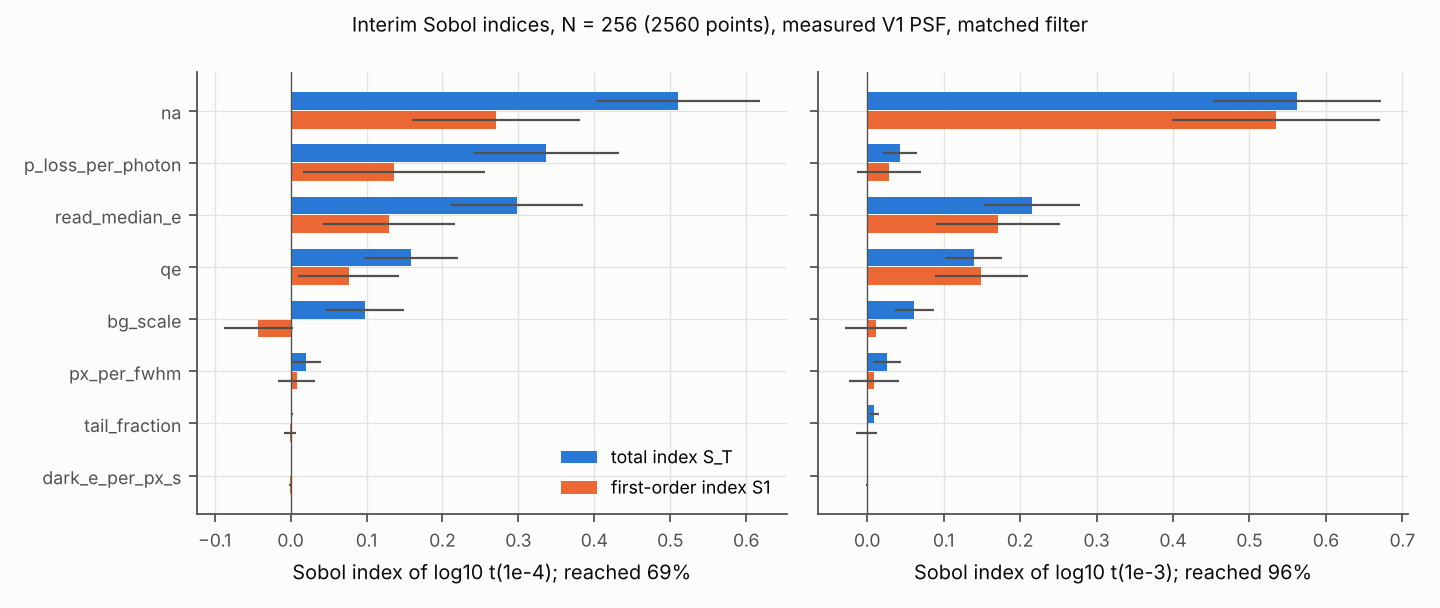
\includegraphics[width=\textwidth]{../figures/prod_sobol_n256.png}
\caption{Sobol indices of $\log_{10} t(10^{-4})$ (left) and $\log_{10} t(10^{-3})$ (right) for the
8-parameter design, $N = 256$ (2560 points), reference scenario with the measured V1 PSF, matched filter.
Bars: total ($S_T$) and first-order ($S_1$) indices; error bars: 95\% bootstrap confidence intervals
(SALib). Parameters ranked by $S_T$ at $10^{-4}$. Points not reaching the target within 1\,s at survival
$\geq 0.99$ (31\% at $10^{-4}$, 4\% at $10^{-3}$) are censored at $\log_{10} t = 0$.}
\label{fig:sobol8}
\end{figure}

\begin{figure}[htbp]
\centering
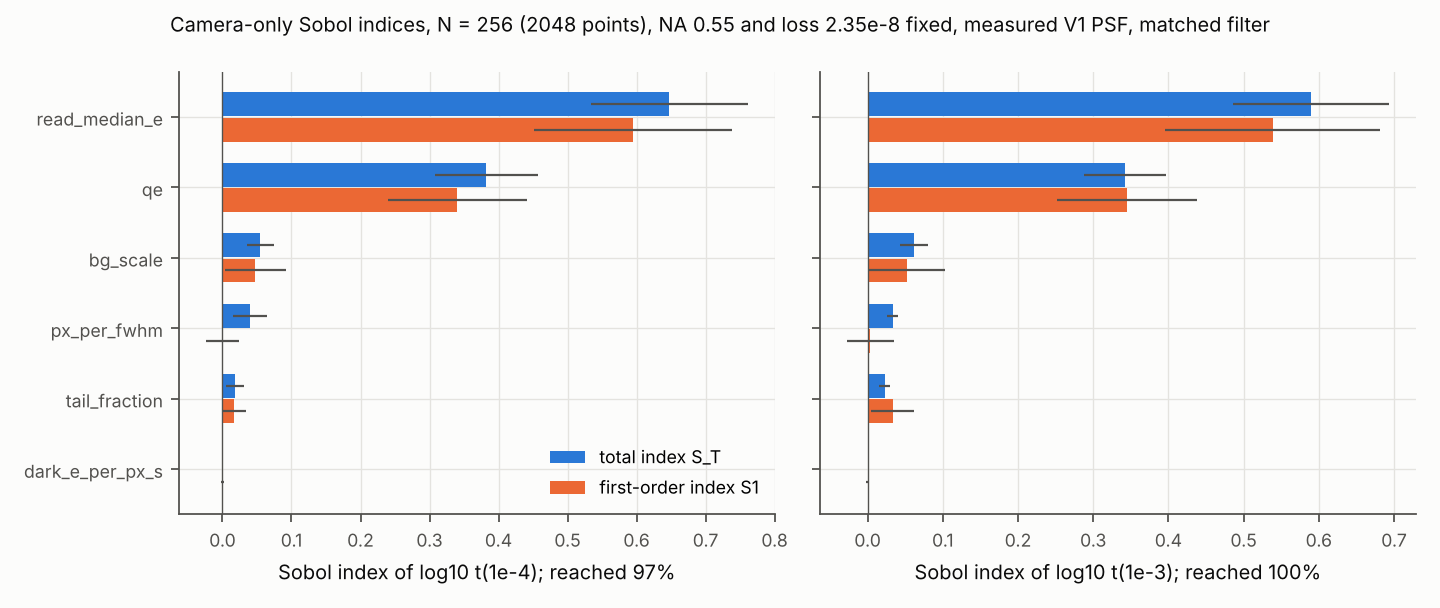
\includegraphics[width=\textwidth]{../figures/prod_sobol_camera_n256.png}
\caption{As Fig.~\ref{fig:sobol8} for the camera-only design: NA 0.55 and loss
$2.35\times10^{-8}$ per photon fixed, six camera-side inputs, $N = 256$ (2048 points), scan to 5\,s
(3\% of points censored at $10^{-4}$, none at $10^{-3}$).}
\label{fig:sobolcam}
\end{figure}

The response is additive (sum of $S_1$ = 0.97 at $10^{-3}$ and 1.00 at $10^{-4}$). However, the ranking
of read noise above QE reflects the sampled ranges: the read-noise range spans a factor of 40 and
includes cameras that are clearly unsuitable, and the log-uniform background range has its median (0.55
of the reference) on the dark side, where read noise weighs more. For a specification, the local
behaviour at a realistic operating point is the relevant quantity (Table~\ref{tab:oppoint}).

\begin{table}[htbp]
\centering
\caption{$t(10^{-3})$ / $t(10^{-4})$ in ms versus read-noise median at the reference background,
1.0\,px per FWHM, no tail, dark current 0.01\,\elec/px/s; same model as the Sobol designs.}
\label{tab:oppoint}
\small
\begin{tabular}{@{}c c c c c c@{}}
\toprule
QE & 0.1\,\elec & 0.25\,\elec & 0.5\,\elec & 1.0\,\elec & 2.0\,\elec \\
\midrule
0.485 & 20.1 / 31.4 & 20.7 / 32.0 & 22.6 / 34.1 & 28.1 / 40.7 & 41.5 / 57.8 \\
0.85 & 11.5 / 17.8 & 11.8 / 18.2 & 12.9 / 19.3 & 16.0 / 23.0 & 23.6 / 32.7 \\
\bottomrule
\end{tabular}
\end{table}

As can be seen from Table~\ref{tab:oppoint}, the read-noise factor relative to 1.0\,\elec{} is the same
at both QE values to within 0.01 (for $10^{-4}$: 0.77, 0.79, 0.84, 1, 1.42; for $10^{-3}$: 0.72, 0.74,
0.80, 1, 1.48), and the QE dependence is $1/\mathrm{QE}$ to within 1\% (DERIVED from
Table~\ref{tab:oppoint}). Hence, at this operating point,
\begin{equation}
  t(10^{-4}) \simeq \SI{40.7}{\milli\second} \times \frac{0.485}{\mathrm{QE}} \times f_4(\sigma_r),
  \label{eq:scaling}
\end{equation}
where $\sigma_r$ is the read-noise median and $f_4$ is the factor above. The same model reproduces the
preset results (Prime BSI Express \SI{41.3}{\milli\second}; ORCA-Quest~2 PNR \SI{39.3}{\milli\second}
against \SI{40.2}{\milli\second} for the preset, whose read-noise model includes a tail class).

\section{Implications}

\paragraph{Stage 1 specification (provisional; reference scenario, matched filter).} Our choice of
requirements is a compromise between imaging time and what a purchased back-illuminated CMOS sensor can
deliver. First, QE at 852\,nm sets the imaging time in proportion: each relative gain in QE shortens the
time by the same factor. Second, a read-noise median of 0.5\,\elec{} or below is within 10\% of an ideal
sensor, whereas 1.0\,\elec{} costs about 30\% and 2.0\,\elec{} about 80\%. Third, pixels with read noise
far above the median must be rare: at a 1.0\,\elec{} median, 2\% of pixels at 5 times the median cost
42\%; the acceptable fraction depends on the measured tail shape, which P4 must supply, and on whether
such pixels can be masked. Fourth, cooling need only keep dark current below about 1\,\elec/px/s, since
the dark charge at 40\,ms is then below 0.04\,\elec{} per pixel (DERIVED); the Sobol designs show no
effect of dark current up to 3\,\elec/px/s. Fifth, the magnification should give 0.5 to 1.4\,px per PSF
FWHM (within 4\% of the best in the camera-only design). The quantitative specification (minimum QE and
maximum read noise for a given time budget) follows from Eq.~\eqref{eq:scaling} once the lab fixes the
imaging-time budget; the generic sweep with the measured PSF (Sec.~\ref{sec:remaining}) will give the
full maps.

\paragraph{Prime BSI Express operating point (provisional).} CMS mode (1.0\,\elec), magnification giving
about 0.7 to 1.0\,px per PSF FWHM (2.7 to 3.8 for the V1 PSF of \SI{1.70}{\micro\metre} FWHM; to be
rescaled with our own measured PSF), matched filter with per-site weights and thresholds:
$t(10^{-3}) = \SI{28.4}{\milli\second}$, $t(10^{-4}) = \SI{41.3}{\milli\second}$, and
$\eps = 1.2\times10^{-4}$ at 40\,ms in the reference scenario. Speed mode costs 19\%
(\SI{49.3}{\milli\second}). A $2048\times128$ region of interest reads out in 1.46\,ms (128 rows at
\SI{11.4}{\micro\second}, USER datasheet line time); with continuous illumination the exposure must
exceed the imaging time by this amount. The read-noise tail of the GSENSE2020BSI is not specified; a
dark-frame stack from our camera is the most useful next input.

\paragraph{Programme level.} At the operating point, raising QE from 0.485 to 0.85 shortens
$t(10^{-4})$ by a factor of 1.77 (Table~\ref{tab:oppoint}). Raising NA from 0.55 to 0.70 increases the
collection fraction by a factor of 1.7 (0.083 to 0.143 for isotropic emission, DERIVED), a comparable
gain from the optics. In our opinion, the case for a custom thick-silicon sensor therefore rests on QE
at 780 and 852\,nm together with cost and supply, and the gain in detection speed alone (about 1.8 times
over a good commercial back-illuminated sensor) should be weighed against an NA upgrade.

\section{Limitations}

(i)~The V1 FP rate is under-predicted 14-fold; if real experiments carry such a floor, camera
improvements below it are invisible. (ii)~Read-noise tails are a two-class model (tail pixels at 3 times
the median for presets with a stated rms, 5 times in the generic and Sobol designs); P4 will replace
this with measured distributions. (iii)~All production results are for one reference scenario: Cs at
852\,nm, NA 0.55, the measured V1 PSF, a uniform background, no neighbour crosstalk, filling 0.5.
(iv)~The characteristic-function engine omits ADC rounding; for the ORCA-Quest~2 in PNR mode exact
rounding lowers $\eps$ by 7\% at the operating point (1 to 2\% in time), so the PNR results are slightly
conservative. (v)~The Sobol results are at $N = 256$, with half-widths of 0.04 to 0.15 on the leading
indices. (vi)~Model~B (Langevin) is used only to bound the effect of the loss-time profile; the
production results use model~A.

\section{Remaining work}
\label{sec:remaining}

\begin{table}[htbp]
\centering
\caption{Outstanding computations and deliverables.}
\label{tab:remaining}
\footnotesize
\begin{tabularx}{\textwidth}{@{}p{4.3cm} p{3.6cm} L@{}}
\toprule
item & size & why it is needed \\
\midrule
generic CMOS sweep with the measured PSF & 725 of 750 points left, at most 19\,CPU-h &
spec-to-fidelity maps in the (QE, read noise) plane consistent with Table~\ref{tab:presets}; the
existing maps use the diffraction-limited PSF \\
full 8-parameter Sobol, $N = 1024$ & 7680 points left, at most about 60\,CPU-h &
halves the confidence intervals; separates NA, loss and read noise at $10^{-4}$ \\
full camera-only Sobol, $N = 1024$ & 6144 points left, at most about 30\,CPU-h &
final ranking of camera parameters for the specification \\
Rb at 780\,nm and the Cs/Rb compromise & not started & required by the brief; QE and PSF differ at 780\,nm \\
neighbour crosstalk and array geometry & not started &
required by the brief; matters when site spacing approaches the PSF width \\
Bayesian per-pixel classifier in production & implemented, validated, not yet in the sweeps &
can exploit a measured read-noise map, the input that matters most after QE \\
EMCCD branch of the generic sweep & not started & EM gain, CIC and frame rate as free parameters \\
written Stage~1 specification and Prime BSI Express recipe & after the items above &
the two deliverables of the brief \\
\bottomrule
\end{tabularx}
\end{table}

The three runs are prepared for the IIT Madras HPC (\file{runs/production/slurm_submit_measpsf.sh},
8 tasks $\times$ 16 cores by default; partition and account [CONFIRM?]). Since the runs above, the
time-to-target scan stops after the last first crossing; re-evaluated points give identical times at
4 to 20 times lower cost, so the sizes in Table~\ref{tab:remaining} are upper bounds.

\section{Computational cost}

\begin{table}[H]
\centering
\caption{CPU time used on the 4-core cloud instance.}
\label{tab:cost}
\small
\begin{tabular}{@{}l r r@{}}
\toprule
study & points & CPU-h \\
\midrule
presets, measured PSF & 77 & 0.66 \\
sensitivity, measured PSF & 26 & 0.17 \\
generic sweep, diffraction-limited PSF & 750 & 7.3 \\
8-parameter Sobol, $N = 256$ & 2560 & 20.3 \\
camera-only Sobol, $N = 256$ & 2048 & 11.0 \\
\bottomrule
\end{tabular}
\end{table}

\FloatBarrier
\begin{thebibliography}{9}
\bibitem{manetsch}
Manetsch, Nomura, Bataille, Leung, Lv and Endres,
``A tweezer array with 6100 highly coherent atomic qubits'',
Nature \textbf{647}, 60--67 (2025), doi:\href{https://doi.org/10.1038/s41586-025-09641-4}{10.1038/s41586-025-09641-4};
text read: arXiv:\href{https://arxiv.org/abs/2403.12021v4}{2403.12021v4}.

\bibitem{picken}
Picken, Legaie and Pritchard,
``Single Atom Imaging with an sCMOS camera'',
Appl.\ Phys.\ Lett.\ \textbf{111} (2017), doi:\href{https://doi.org/10.1063/1.5003304}{10.1063/1.5003304};
text read: arXiv:\href{https://arxiv.org/abs/1709.00946v2}{1709.00946v2}.

\bibitem{basden}
Basden, Haniff and Mackay,
``Photon counting strategies with low light level CCDs'',
Mon.\ Not.\ R.\ Astron.\ Soc.\ \textbf{345}, 985--991 (2003),
doi:\href{https://doi.org/10.1046/j.1365-8711.2003.07020.x}{10.1046/j.1365-8711.2003.07020.x};
text read: arXiv:\href{https://arxiv.org/abs/astro-ph/0307305v1}{astro-ph/0307305v1}.

\bibitem{steck}
Steck, ``Cesium D Line Data'', revision 2.3.4 (2025),
\url{https://steck.us/alkalidata/cesiumnumbers.pdf}.

\bibitem{salib}
SALib, Sensitivity Analysis Library in Python, version 1.6.0, \url{https://github.com/SALib/SALib}.
\end{thebibliography}

\appendix
\section{Provenance ledger (principal values)}

{\footnotesize
\begin{tabularx}{\textwidth}{@{}p{4.9cm} >{\raggedright\arraybackslash}p{2.0cm} >{\raggedright\arraybackslash}p{1.6cm} L@{}}
\toprule
value & location & type & pointer \\
\midrule
FN $5.50\times10^{-5}$, FP $7.01\times10^{-5}$, fidelity 0.9999374(8), QE 0.44, 2.7\%, 80\,ms, NA 0.55 &
Sec.~2, 3 & SOURCE & Ref.~\cite{manetsch}, arXiv:2403.12021v4 (main text and Methods) \\
readout error $< 8\times10^{-7}$, 40\,ms, Zyla 5.5 & Sec.~2 & SOURCE & Ref.~\cite{picken}, arXiv:1709.00946v2 \\
$F^2 = 1/g + 2/g^{1/r} - 2/g^{1+1/r}$ & Sec.~2 & SOURCE & Ref.~\cite{basden}, Eq.~5 (\file{sources/README.md}) \\
FN $4.91\times10^{-5}$ to $5.73\times10^{-5}$, FP $4.85\times10^{-6}$, gains 0.381 / 0.368\,\elec/ADU, $F^2 = 1.972$ &
Table~\ref{tab:validation} & SIM & \file{runs/validation/}, \file{reports/p1_validation.md} (review before submission) \\
rate \SI{72.3e3}{\per\second}, $\eta_\mathrm{opt}$ 0.327, loss $2.35\times10^{-8}$, background 4.76\,\elec/px/s &
Sec.~3 & DERIVED / DATA & \file{configs/production/reference_cs.yaml} pointers \\
PSF $1/e^2$ radius \SI{1.44}{\micro\metre}, FWHM \SI{1.70}{\micro\metre}; vectorial FWHM \SI{0.82}{\micro\metre} &
Sec.~3 & DERIVED & \file{reference_cs.yaml}; \file{optics/array.py} (PSFSpec.fwhm) \\
survival $\geq 0.99$ up to 5.9\,s & Sec.~3 & DERIVED & $0.01005/(2.35\times10^{-8}\times\SI{72.3e3}{\per\second})$ \\
QE at 852\,nm per preset & Table~\ref{tab:presets} & DATA / USER & \file{camsim_common/presets/*.yaml} (digitised vendor curves; USER-supplied PDFs) \\
preset times, magnifications & Table~\ref{tab:presets}, Fig.~\ref{fig:presets} & SIM &
\file{runs/production/prod_presets/}, \file{prod_presets_difflim/} (review before submission) \\
sensitivity times & Table~\ref{tab:sensitivity} & SIM & \file{runs/production/prod_sensitivity/} (review before submission) \\
loss bound $5.6\times10^{-7}$ & Table~\ref{tab:sensitivity} & DERIVED &
Ref.~\cite{picken}: retention $> 99\%$ at 450 photons/ms, 40\,ms (\file{configs/production/sensitivity.yaml}) \\
8-parameter Sobol indices & Sec.~6, Fig.~\ref{fig:sobol8} & SIM & \file{runs/production/prod_sobol/points/}, rows 0 to 2559 (review before submission) \\
camera-only Sobol indices & Table~\ref{tab:sobolcam}, Fig.~\ref{fig:sobolcam} & SIM &
\file{runs/production/prod_sobol_camera/points/}, rows 0 to 2047 (review before submission) \\
operating-point times & Table~\ref{tab:oppoint} & SIM &
\file{p1_atomdet.sweep.evaluate.sobol_point} with \file{configs/production/sobol_camera.yaml} (review before submission) \\
read-noise factors, $1/\mathrm{QE}$ scaling, Eq.~\eqref{eq:scaling} & Sec.~6 & DERIVED & ratios of Table~\ref{tab:oppoint} entries \\
collection fraction 0.023, 0.083, 0.143, 0.200 at NA 0.3, 0.55, 0.7, 0.8 & Sec.~6, 7 & DERIVED &
$(1-\sqrt{1-\mathrm{NA}^2})/2$, isotropic emission (\file{optics/collection.py}) \\
line time \SI{11.4}{\micro\second} (CMS) & Sec.~7 & USER & Prime BSI Express datasheet rev.\ 2024-08-20 \\
CPU time & Table~\ref{tab:cost} & DATA & per-point cost records in the run directories \\
\bottomrule
\end{tabularx}
}

\section{Open placeholders}

The presets carry 116 open [VALUE?] entries (full list in \file{reports/p1_production_note.md}). Of
these, 40 belong to the two validation presets and the model-B parameters and are discussed in
\file{reports/p1_validation.md}; 76 belong to the eleven production presets. The production engine does
not read 54 of the 76 (cosmic-ray parameters, PRNU, ADC offset, line time). The remaining 22 can affect
the results above: (i)~read-noise median or rms where the vendor states a single value (6 entries; sets
the tail class of the preset); (ii)~dark-current parameters (7; negligible by Sec.~\ref{sec:sobol}
unless dark current exceeds about 1\,\elec/px/s); (iii)~EMCCD register length and CIC split (4; the
split is swept in Table~\ref{tab:sensitivity}); (iv)~ADC parameters (5; ADC rounding is omitted by the
production engine). In addition, the SLURM partition and account are [CONFIRM?].

\end{document}
